% =========================
% Figure: egp_contribs
% Shows both D-normalized terms and (1-alpha) weighted-sum terms
% =========================
% Preamble needs:
% \usepackage{pgfplots}
% \pgfplotsset{compat=1.18}
\begin{figure}[htbp]
\centering
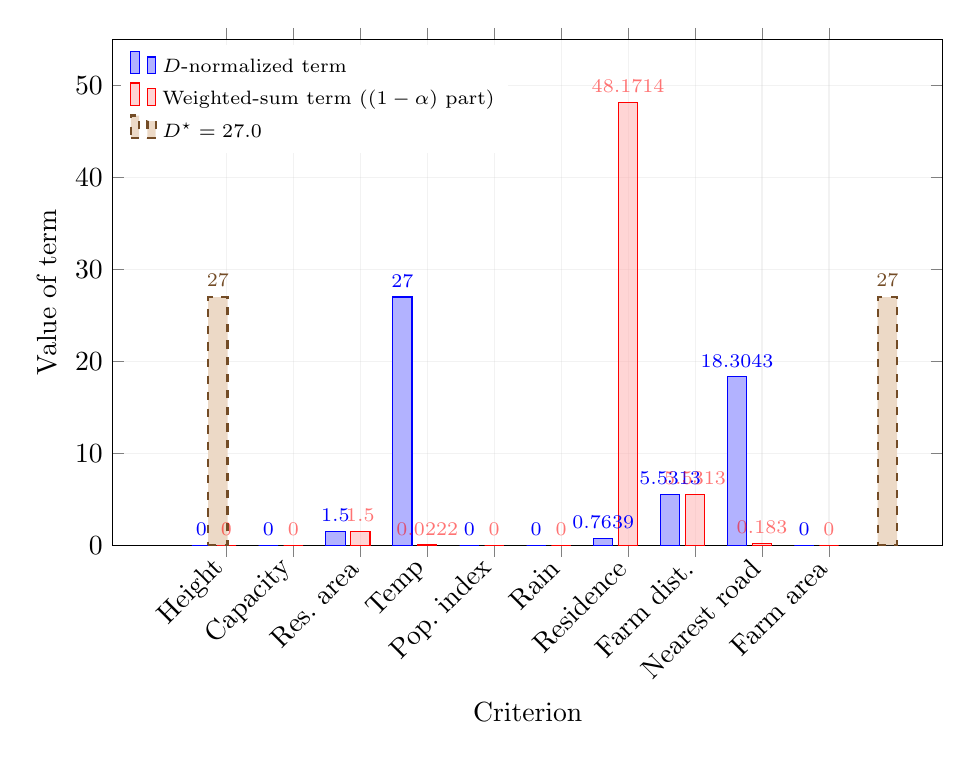
\begin{tikzpicture}
\begin{axis}[
    ybar,
    width=\textwidth,
    height=8cm,
    ymin=0,
    ymax=55, % accommodates the large p7/0.35 bar
    bar width=7pt,
    enlarge x limits=0.12,
    xlabel={Criterion},
    ylabel={Value of term},
    xtick=data,
    xticklabel style={rotate=45, anchor=east},
    xticklabels={
      Height,
      Capacity,
      Res.~area,
      Temp,
      Pop.~index,
      Rain,
      Residence,
      Farm~dist.,
      Nearest~road,
      Farm~area
    },
    legend style={draw=none, at={(0.01,0.99)}, anchor=north west, font=\scriptsize},
    legend cell align={left},
    nodes near coords,
    nodes near coords align={vertical},
    every node near coord/.append style={font=\scriptsize, /pgf/number format/fixed, /pgf/number format/precision=4},
    grid=both,
    grid style={opacity=0.2}
]
% --- Series 1: D-normalized terms (from the D-constraints) ---
% n1/47=0, n2/3=0, p3/0.04=1.5, p4/0.04=27.0, n5/48.74=0, n6/0.52=0,
% p7/22.07≈0.7639, p8/0.32=5.5313, p9/0.23≈18.3043, n10/0.68=0
\addplot+[fill] coordinates {
 (1,0.0000) (2,0.0000) (3,1.5000) (4,27.0000) (5,0.0000)
 (6,0.0000) (7,0.7639) (8,5.5313) (9,18.3043) (10,0.0000)
};
\addlegendentry{$D$-normalized term}

% --- Series 2: (1-$\alpha$) weighted-sum terms in the EGP objective ---
% Only present for p3, p4, p7, p8, p9 (others are zero here)
% p3/0.04=1.5, p4/48.74≈0.0222, p7/0.35≈48.1714, p8/0.32=5.5313, p9/23≈0.1830
\addplot+[fill, fill opacity=0.55] coordinates {
 (1,0.0000) (2,0.0000) (3,1.5000) (4,0.0222) (5,0.0000)
 (6,0.0000) (7,48.1714) (8,5.5313) (9,0.1830) (10,0.0000)
};
\addlegendentry{Weighted-sum term ($(1-\alpha)$ part)}

% Reference line at D*
\addplot+[domain=0.5:10.5, samples=2, thick, dashed] {27.0};
\addlegendentry{$D^{\star}=27.0$}
\end{axis}
\end{tikzpicture}
\caption{EGP contributions by criterion: comparison of the $D$-normalized terms (used in the minimax bound) versus the terms entering the $(1-\alpha)$ weighted-sum portion of the objective ($\alpha=0.8$). The $D$-binding criterion is \emph{Temperature}; the weighted-sum is dominated by \emph{Residence}.}
\label{fig:egpDeviations}
\end{figure}
